\documentclass[
12pt, % 字体大小
a4paper, 
oneside, % 单面打印(双面为twoside)
headinclude,footinclude, % 页眉页脚包含在文本区域内,确保不被裁剪或掩盖
]{scrartcl}
% 主题和样式
\usepackage[
nochapters, % 无章节层级 
beramono, % 等宽字体样式
eulermath, % 数学公式Euler字体
pdfspacing, % 字间距
dottedtoc % 点线式目录
]{classicthesis}
\usepackage{arsclassica} 
%----------------------------------------------------------------------------------------
% 输入和页面排版
\usepackage[T1]{fontenc} % 字体编码
\usepackage[utf8]{inputenc} % 输入编码
\usepackage{ctex} % 汉语
\usepackage{amsmath,amssymb,amsthm} % 数学公式
\usepackage{indentfirst} % 缩进
\setlength{\parindent}{2em} % 段落缩进
\usepackage[
top=2cm,
bottom=2cm, 
left=2cm,
right=2cm, 
headheight=20pt, 
includeheadfoot 
]{geometry} % 页面
\usepackage{scrlayer-scrpage} % 页眉页脚
\renewcommand{\sectionmark}[1]{\markright{\spacedlowsmallcaps{#1}}}
\renewcommand{\subsectionmark}[1]{\markright{\thesubsection~#1}}
\lehead{\mbox{\llap{\small\thepage\kern1em\color{halfgray} \vline}\color{halfgray}\hspace{0.5em}\rightmark\hfil}} % 标题旁边标记页码
\cfoot{\hyperlink{toc}{\color{RoyalBlue}返回目录}} % 页脚返回目录链接
\pagestyle{scrheadings}
%----------------------------------------------------------------------------------------
% 图表和引用
\usepackage{graphicx} % 图像
\graphicspath{{Figures/}} % 图像路径
\usepackage{subfig} % 图组
\usepackage{float} % 浮动
\usepackage{enumitem} % 列表
\usepackage{varioref} % 交叉引用
%----------------------------------------------------------------------------------------
% 代码
\usepackage{listings}
\lstset{
    language=Matlab,
    basicstyle=\ttfamily\small,   % 字体
    numbers=left,                 % 行号
    numberstyle=\tiny\color{gray},
    stepnumber=5,
    numbersep=5pt,
    backgroundcolor=\color{white},% 背景
    tabsize=2,                    % 制表符宽度
    frame=single,                 % 边框
    captionpos=t,                 % 标题
    title=\lstname,
    breaklines=true,              % 换行
    breakatwhitespace=true,
    escapeinside={`}{`},          % 转义(中文注释)
}
\lstset{
    language=Python,            
    basicstyle=\ttfamily\small,   % 字体
    numbers=left,                 % 行号
    numberstyle=\tiny\color{gray}, 
    stepnumber=5,             
    numbersep=5pt,            
    backgroundcolor=\color{white},% 背景
    tabsize=4,                    % 制表符宽度            
    frame=single,                 % 边框
    captionpos=t,                 % 标题
    title=\lstname, 
    breaklines=true,              % 换行
    breakatwhitespace=false,   
    escapeinside={`}{`},          % 转义(中文注释)
}
\usepackage{algorithm} % 算法
\usepackage{algpseudocode}
\usepackage{mdframed} % 跨页框架
% 不浮动算法环境
\newcounter{myalgorithm}
\renewcommand{\themyalgorithm}{\arabic{myalgorithm}}
\newenvironment{myalgorithm}[1][]{
  \refstepcounter{myalgorithm}
  \begin{mdframed}[
    skipabove=\topskip,
    skipbelow=\topskip,
    needspace=3\baselineskip,
    linewidth=0.4pt,
    frametitlefont=\normalfont\bfseries,
    frametitle={算法 \themyalgorithm\if\relax\detokenize{#1}\relax\else:#1\fi},
    frametitlerule=true,
    frametitlerulewidth=0.4pt,
    repeatframetitle=true
  ]
  \begin{algorithmic}[1]
  \ifx\relax\detokenize{#1}\relax
    \addcontentsline{alg}{algorithms}{\makebox[7em][l]{算法~\themyalgorithm} }
  \else
    \addcontentsline{alg}{algorithms}{\makebox[7em][l]{算法~\themyalgorithm} #1}
  \fi
}{
  \end{algorithmic}
  \end{mdframed}
}
% 关键词
\algrenewcommand{\algorithmicwhile}{当}
\algrenewcommand{\algorithmicdo}{执行}
\algrenewcommand{\algorithmicend}{结束}
\algrenewcommand{\algorithmicif}{如果}
\algrenewcommand{\algorithmicthen}{那么}
\algrenewcommand{\algorithmicelse}{否则}
\algrenewcommand{\algorithmicfor}{对于}
\algrenewcommand{\algorithmicrepeat}{循环}
\algrenewcommand{\algorithmicuntil}{直到}
\algrenewcommand{\algorithmicloop}{循环}
\algnotext{EndFor}
\algnotext{EndIf}
\algnotext{EndLoop}
\algnotext{EndWhile}
%----------------------------------------------------------------------------------------
% 超链接与PDF信息
\usepackage{hyperref} 
\hypersetup{
colorlinks=true, % 彩色
breaklinks=true, % 断行
urlcolor=webbrown, % URL棕色
linkcolor=RoyalBlue, % 内部链接蓝色
citecolor=webgreen, % 引用绿色
bookmarks=true, % 书签
bookmarksnumbered,
pdftitle={}, 
pdfauthor={},
pdfsubject={}, 
pdfkeywords={}, 
pdfcreator={pdfLaTeX}, 
pdfproducer={LaTeX with hyperref and ClassicThesis} 
}
%----------------------------------------------------------------------------------------
% 目录与标题
\usepackage{titlesec} 
\AtBeginDocument{
    \renewcommand{\contentsname}{目\hspace{1em}录}
    \renewcommand{\listfigurename}{图\hspace{1em}片}
    \renewcommand{\listtablename}{表\hspace{1em}格}
    \renewcommand{\figurename}{图}
    \renewcommand{\tablename}{表}
    \setcounter{tocdepth}{3} % 目录深度
}
\theoremstyle{definition} 
\newtheorem{definition}{定义}
\theoremstyle{plain} 
\newtheorem{theorem}{定理}
\theoremstyle{remark}
\newtheorem{remark}{备注}
\newtheorem{example}{样例}
\usepackage{tocloft} % 目录
% 要点目录
\newlistof{tips}{tip}{要\hspace{1em}点}
\newcommand{\tip}[1]{
  \refstepcounter{tips}
  \textsuperscript{\textcolor{orange}{\textbf{\thetips}}}
  \addcontentsline{tip}{tips}{\makebox[7em][l]{要点~\thetips} #1}
}
% 算法目录
\newlistof{algorithms}{alg}{算\hspace{1em}法} 
\hyphenation{Fortran hy-phen-ation} % 单词断字规则
%----------------------------------------------------------------------------------------
% 题目和作者
\title{\normalfont\spacedallcaps{深度学习}} 
\date{}
%----------------------------------------------------------------------------------------
% 开始和目录
\begin{document}
\maketitle
\newpage
\hypertarget{toc}{}
\begingroup
\begin{multicols}{2}
\tableofcontents
\end{multicols}
\endgroup
\hrule
\begingroup
\begin{multicols}{2}
\listoffigures
\end{multicols}
\endgroup
\hrule
\begingroup
\begin{multicols}{2}
\listoftables
\end{multicols}
\endgroup
\newpage
%----------------------------------------------------------------------------------------
\section{学术史}
\begin{table}[H]
\centering
\begin{tabular}{|l|c|c|}
\hline
姓名 & 图灵奖 & 诺贝尔奖 \\
\hline
Geoffrey Hinton & $ \surd $ & $ \surd $ \\
\hline
John Hopfield & $ x $ & $ \surd $ \\
\hline
\end{tabular}
\caption{奖项获得情况}
\end{table}
%----------------------------------------------------------------------------------------
\section{神经网络}
%------------------------------------------------
\subsection[概念]{概念}
深度学习的“深度”:神经网络的深度(层数)。
%------------------------------------------------
\paragraph{数据集}
\begin{itemize}
\item 训练集。
\item 测试集。
\item 验证集。
\end{itemize}
%------------------------------------------------
\paragraph{参数}
\begin{itemize}
\item 超参数:网络层数、学习率(策略)、批量大小。不能只在训练集或测试集上获得,要通过训练和验证获得。
\item 非超参数:网络权重(不唯一,比如倍数)。
\end{itemize}
%------------------------------------------------
\subsection[前馈神经网络]{前馈神经网络(Feed-Forward Neural Network,FNN)}
相邻层间特征单向连接。

\begin{figure}[H]
\centering 
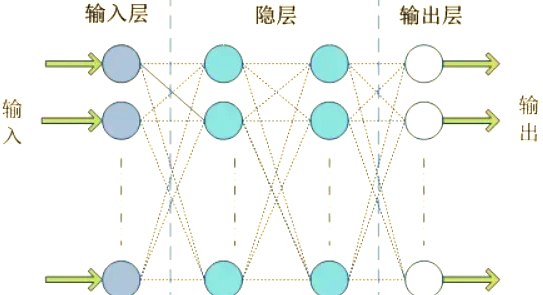
\includegraphics[width=0.4\textwidth]{fnn} 
\caption{前馈神经网络}
\end{figure}
%------------------------------------------------
\paragraph{全连接神经网络(Full Connect Neural Network,FCNN)}
\begin{itemize}
\item 前向传播:计算结果并保存特征。
\item 反向传播:链式规则。
\end{itemize}
%------------------------------------------------
\subsection[卷积神经网络]{卷积神经网络(Convolutional Neural Networks,CNN)}
%------------------------------------------------
\subsubsection[结构]{结构}
\begin{itemize}
\item 卷积层:提取局部特征。
\item 池化层:降低特征维度。
\item 全连接层:分类。
\end{itemize}

\begin{figure}[H]
\centering 
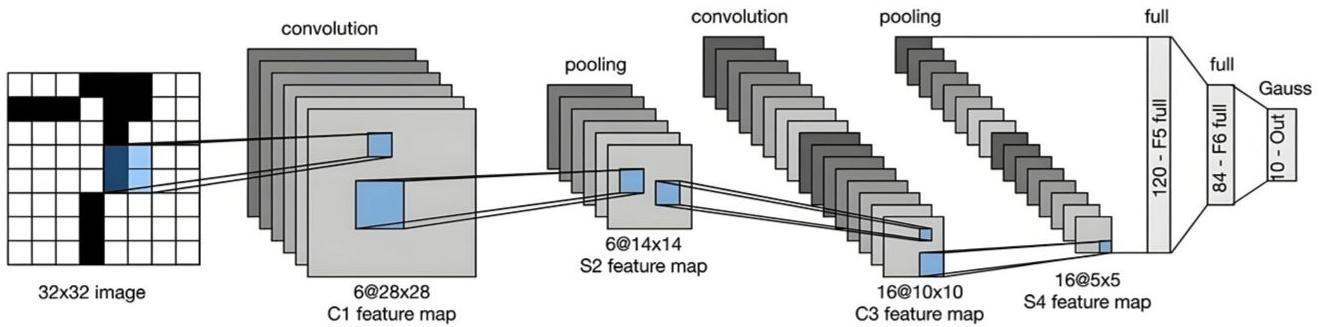
\includegraphics[width=0.8\textwidth]{cnn} 
\caption{卷积神经网络}
\end{figure}
%------------------------------------------------
\paragraph{卷积}~\\

计算:
\begin{itemize}
\item 原图像:$ H_0 \times N_0 \times M_0 \times A_0 $。
\item 卷积核:$ B \times F \times F \times A_0 $。
\item 填充:$ P $。
\item 步幅:$ S $。
\item 新图像大小:$ N_1 = \frac{N_0 + 2P - F}{S} + 1, A_1 = B $。
\item 参数量:$ F \times F \times A_0 \times B $。
\end{itemize}

$ 1 \times 1 $卷积:
\begin{itemize}
\item 维度变换(降/升维):改变特征图的深度(通道数)。降维有助于降低模型复杂度和计算量,同时保持大部分有用信息。
\item 非线性引入:在卷积后添加激活函数,可以在不改变空间尺寸的情况下引入非线性,使模型能够学习更复杂的模式。
\item 作为瓶颈层:在一些架构(如ResNet、Inception)中,可以用作瓶颈层(先降维,再进行其他卷积,最后恢复维度)。显著减少参数量和计算成本,同时维持性能。
\item 特征融合:融合不同尺度或不同来源的特征图,合并成一个新的特征表示。
\end{itemize}
%------------------------------------------------
\paragraph{池化}
参数量为$ 0 $,计算区域的代表性特征值。
\begin{itemize}
\item 最大池化(Max Pooling):最大值。
\item 平均池化(Average Pooling):平均值。
\end{itemize}
%------------------------------------------------
\paragraph{填充(Padding)}
\begin{itemize}
\item 增加感受野,减少信息损失:确保边缘像素能被卷积核充分覆盖,得到有效处理,而不是丢失。
\item 控制输出尺寸:通过调整填充量可以精确控制每一层的输出尺寸。
\end{itemize}
%------------------------------------------------
\paragraph{步幅(Stride)}
\begin{itemize}
\item 控制输出尺寸、下采样程度:较大步幅可以减小输出的空间尺寸,降低计算复杂度,减少参数量,提高特征图的缩放比例。
\item 调整感受野:较大步幅时输出单元会覆盖较大输入区域,增加感受野,减少重叠区域数量。
\item 平衡速度与精度:较大步幅可加速计算过程,但可能丢失细节信息;较小步幅能更精细地捕捉特征,但会增加计算成本。
\end{itemize}
%------------------------------------------------
\subsubsection[实例]{实例}
趋势:卷积核变小、层数增加,抛弃池化层、全连接层。
\begin{itemize}
\item LeNet:没有使用ReLU。
\item AlexNet:最早使用了ReLU、GPU。
\item VGGNet:小卷积核(感受野上,$ 3 \times 3 \times 3  = 1 \times 7 \times 7 $)。
\item GoogleNet:使用了ReLU,Inception。$ 1 \times 1 $卷积。
\item ResNet:使用了ReLU,恒等映射直连边,残差模块。
\end{itemize}
%------------------------------------------------
\section[问题与改进]{问题与改进}
%------------------------------------------------
\subsection[问题]{问题}
%------------------------------------------------
\subsubsection[拟合]{拟合}
\begin{table}[H]
\centering
\begin{tabular}{|p{1.5cm}|p{8.5cm}|p{2cm}|p{2cm}|}
\hline
问题 & 描述 & \multicolumn{2}{|c|}{训练收敛的网络} \\
\cline{3-4}
 &  & 训练误差 & 测试误差 \\
\hline
欠拟合 & 未训练收敛 & 大 & 大 \\
\hline
过拟合 & 在训练集上表现良好,但不能推广到测试集 & 小 & 大 \\
\hline
\end{tabular}
\caption{欠拟合和过拟合}
\end{table}
%------------------------------------------------
\subsubsection[梯度]{梯度}
\begin{table}[H]
\centering
\begin{tabular}{|p{0.5cm}|p{3.5cm}|p{3.5cm}|p{8cm}|}
\hline
 & 定义 & 问题 & 改善方法 \\
\hline
梯度消失 & 网络层数增加,反向传播过程中梯度逐渐变小,甚至趋于零。 & 权重更新缓慢,甚至停止更新,影响模型的学习能力,使网络难以训练。 & 使用ReLU及其变体。 \newline 采用批量规范化。 \newline 选择Xavier初始化或He初始化)。 \\
\hline
梯度爆炸 & 反向传播过程中梯度变得非常大。 & 权重更新过大,模型学习过程不稳定,甚至发散,无法收敛到最优解。 & 使用ReLU及其变体。 \newline 采用梯度裁断。 \newline 使用Adam优化器。 \newline 采用批量规范化,稳定梯度,减小影响。 \\
\hline
\end{tabular}
\caption{梯度消失和梯度爆炸}
\end{table}
%------------------------------------------------
\subsection[改进技术]{改进技术}
%------------------------------------------------
\subsubsection[损失函数]{损失函数}
交叉熵损失函数更适用于分类问题,常用于衡量模型预测的概率分布与真实标记的概率分布之间的差异。
%------------------------------------------------
\subsubsection[激活函数]{激活函数}
\begin{table}[H]
\centering
\begin{tabular}{|p{2cm}|p{5.5cm}|p{4.5cm}|p{4.5cm}|}
\hline
激活函数 & 函数 & 优点 & 缺点 \\
\hline
ReLU & $ y = \max(0, x) \newline y' = \begin{cases} 1, & z > 0 \\ 0, & z \leq 0 \end{cases} $ & 计算简单,收敛快。解决了梯度消失问题,允许误差迅速回传。有助于稀疏激活,更简洁且减少过拟合风险。 & 存在死区问题(神经元输入小于$ 0 $时将永远不被激活)。 \newline 非零中心化,导致下一层权重更新不均衡。 \\
\hline
Sigmoid & $ y = \frac{1}{1 + e^{-z}} \newline y' = y(1 - y)' $ & 输出范围固定在$ (0, 1) $,适用于二分类问题。函数平滑且处处可微,有利于梯度计算。 & 非零中心化,正输出,减慢收敛速度。 \newline 计算成本高。 \\
\hline
Softmax & 对单个定义$ y = e^x $ \newline $ y(x_i) = \frac{e^{x_i}}{\sum_{i = 1}^n e^{x_i}} $ & 适用于多分类问题。 & 存在数值溢出问题,不适合隐藏层。 \\
\hline
Tanh & $ y = \frac{e^x - e^{-x}}{e^x + e^{-x}} $ & 零中心化输出,收敛性能好,适用于二分类问题。 & 易饱合,梯度消失。 \\
\hline
Leaky ReLU & $ y = \max(0.1x, x) $ & & \\
\hline
ELU & $ y = \begin{cases} x, & x \geq 0 \\ a(e^x - 1), & x < 0 \end{cases} $ & & \\
\hline
Maxout & $ y = \max(w_1^T x + b_1, w_2^T x + b_2) $ & & \\
\hline
\end{tabular}
\caption{激活函数对比}
\end{table}

\begin{figure}[H]
\centering
\subfloat[ReLU]{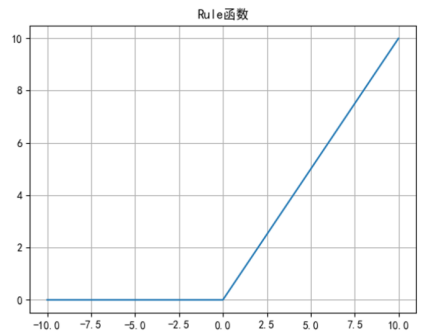
\includegraphics[width=.3\textwidth]{relu}} \quad
\subfloat[Sigmoid]{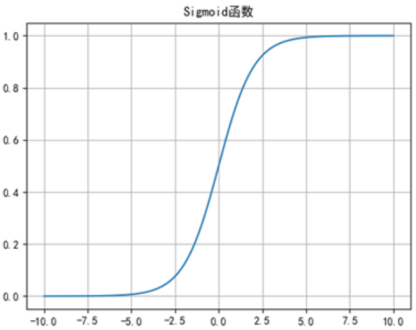
\includegraphics[width=.3\textwidth]{sigmoid}} \quad
\subfloat[Softmax]{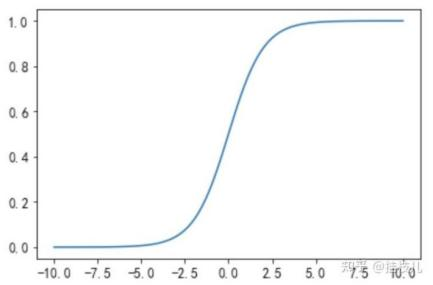
\includegraphics[width=.3\textwidth]{softmax}} \\
\subfloat[Tanh]{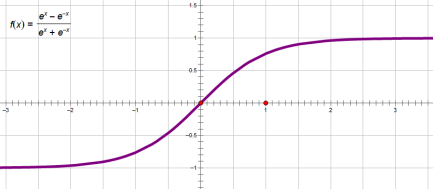
\includegraphics[width=.3\textwidth]{tanh}} \quad
\subfloat[Leaky ReLU]{\includegraphics[width=.3\textwidth]{leakyreLU}} \quad
\subfloat[ELU]{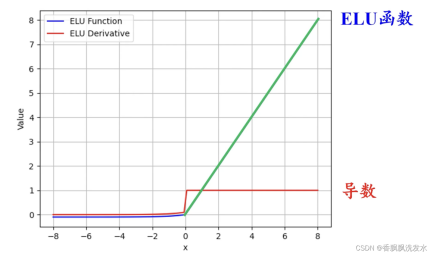
\includegraphics[width=.3\textwidth]{elu}}
\caption{激活函数图像}
\end{figure}
%------------------------------------------------
\paragraph{ReLU与Sigmoid对比}
\begin{itemize}
\item ReLU优点:
\begin{itemize}
\item 梯度问题:ReLU在正区间内不会导致梯度消失;Sigmoid容易陷入饱和区,在区域内梯度几乎为零,导致梯度消失。
\item 计算效率:ReLU只需判断输入是否大于$ 0 $,Sigmoid涉及指数运算。
\item 稀疏激活:ReLU有助于产生稀疏激活,使模型更简洁,减少过拟合风险。
\item 收敛速度:ReLU可使随机梯度下降更快收敛。
\end{itemize}
\item Sigmoid优点:
\begin{itemize}
\item 输出范围:Sigmoid将输入映射到$ (0, 1) $,对特定任务(如二分类问题)更有效。
\item 适用于特定架构或任务:在RNNs中,Sigmoid被用于门控机制,控制信息流。
\item 非线性表达能力:Sigmoid在定义域上平滑且处处可微,非线性表达能力强。
\end{itemize}
\end{itemize}
%------------------------------------------------
\subsubsection[优化器]{优化器}
\begin{itemize}
\item 二阶算法,牛顿法。
\item SGD。
\item SGD + Momentum。
\item ADam。
\item ADamW。
\end{itemize}
%------------------------------------------------
\subsubsection[权重初始化]{权重初始化}
\begin{table}[H]
\centering
\begin{tabular}{|p{3cm}|p{5cm}|p{6cm}|}
\hline
方法 & 特点 & 优点 \\
\hline
高斯分布随机初始化 & 基于正态分布,零均值有方差。 & 确保信号在传播中既不会迅速消失也不会爆炸。 \\
\hline
Xavier初始化 & \multirow{2}{5cm}{确保前向、反向传播过程中激活值和梯度方差保持一致。} & 适用于使用Tanh或Sigmoid的网络。 \\
\cline{1-1}\cline{3-3}
Kaiming均匀分布初始化(He初始化) & & 适用于使用ReLU及其变体的网络。 \\
\hline
\end{tabular}
\caption{权重初始化方法对比}
\end{table}
%------------------------------------------------
\subsubsection[正则化]{正则化}
\begin{itemize}
\item 丢弃法(dropout):在训练过程中随机失活部分神经元(输出$ 0 $),减少对训练集的过度依赖,阻止特征间自适应。可以防止过拟合,提高鲁棒性,间接减小计算量,实现模型平均效果。
\item L1正则化:使权重稀疏。
\item L2正则化:是权重分散。
\end{itemize}
%------------------------------------------------
\subsubsection[训练策略/技巧]{训练策略/技巧}
\begin{itemize}
\item 批量规范化(Batch Normalization):归一化每个小批量样本为标准正态分布,减少梯度消失和梯度爆炸问题,加速收敛。提高模型稳定性、泛化能力,减少对其他正则化技术的依赖。
\item 早停。
\item 梯度裁断(Gradient Clipping):限制梯度大小,防止其变得过大
\end{itemize}
%----------------------------------------------------------------------------------------
\section{循环神经网络}
%------------------------------------------------
\subsection[典型网络]{典型网络}
%------------------------------------------------
\subsubsection[RNN]{RNN(Recurrent Neural Network,循环神经网络)}
循环核计算:
\begin{itemize}
\item 隐藏状态更新:$ h_t = f_w(h_{t - 1}, x_t) = \tanh(w_{xh}x_t + w_{hh}h_{t - 1} + b_h) $。
\item 输出生成:$ y_t = f_{why}(h_t) = Softmax(w_{hy}h_t + b_y) $。
\end{itemize}

\begin{figure}[H]
\centering
\subfloat[RNN]{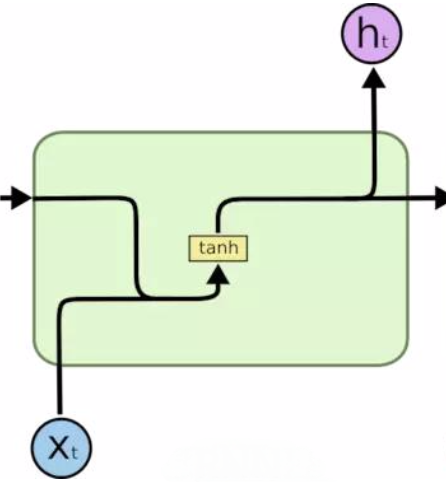
\includegraphics[width=.2\textwidth]{rnn}} \quad
\subfloat[GRU]{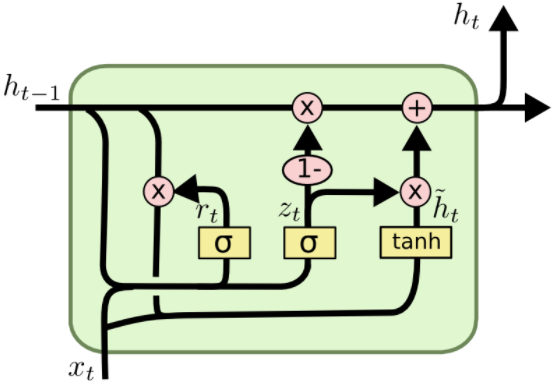
\includegraphics[width=.3\textwidth]{gru}} 
\caption{RNN与GRU更新单元}
\end{figure}
%------------------------------------------------
\subsubsection[GRU]{GRU(Gated Recurrent Unit networks,门控循环单元网络)}
重置门和更新门,没有细胞状态。相比于RNN,主要改善了梯度消失问题。
%------------------------------------------------
\subsubsection[LSTM]{LSTM(Long Short-Term Memory networks,长短期记忆网络)}
遗忘门、输入门、输出门中使用Sigmoid激活函数。
\begin{itemize}
\item 细胞状态(Cell State,黄色):贯穿模型,根据遗忘门和输入门的结果,在整个序列上进行少量的线性交互,使信息流动而不发生太多改变。
\item 遗忘门(Forget Gate,红色):决定从细胞状态中丢弃的信息,查看前一时刻的隐藏状态和当前输入,输出$ [0, 1] $的值给细胞状态的每个元素。$ 0 $意味着完全丢弃,$ 1 $意味着完全保留。
\item 输入门(Input Gate,蓝色):,包含一个用于确定要更新部分的Sigmoid层,和一个创建新候选值向量的Tanh层。 
\item 输出门(Output Gate,绿色):决定细胞状态的输出。Sigmoid层决定细胞状态的输出部分,Tanh层缩放细胞状态,与Sigmoid门的输出相乘,得到本时刻输出。
\end{itemize}

\begin{figure}[H]
\centering 
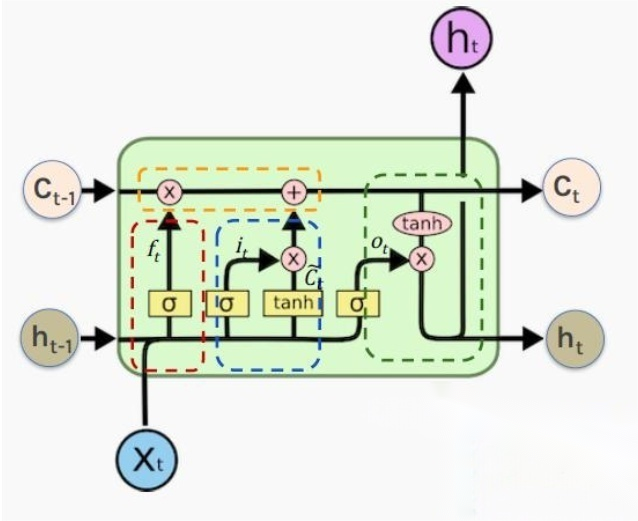
\includegraphics[width=0.4\textwidth]{lstm} 
\caption{LSTM更新单元}
\end{figure}
%------------------------------------------------
\section{Transformer}
%------------------------------------------------
\subsection[注意力机制]{注意力机制}
%------------------------------------------------
\paragraph{组件}
\begin{itemize}
\item 键(Key)。
\item 值(Value)。
\item 查询(Query)。
\end{itemize}
%------------------------------------------------
\paragraph{多头自注意力(Multi-Head Self-Attention)}
\begin{enumerate}
\item 对于输入序列$ X = [x_1, x_2, \ldots, x_n] $,其维度是$ [n, d_{model}] $。
\item 由权重矩阵$ W^Q,  W^K, W^V $生成查询、键、值,维度是$ [d_{model}, d_k], d_k < d_{model} $:
$$ Q = X W^Q, \quad K = X W^K, \quad V = X W^V $$
\item 将其分割成$ h $个头,每个头维度为$ \frac{d_k}{h} $:
$$ Q_{split} = Split(Q), \quad K_{split} = Split(K), \quad V_{split} = Split(V) $$
\item 对每个头计算注意力分数(点乘查询与键,$ d_k $ 缩放,$ Softmax $,加权求和):
$$ Attention(Q, K, V) = Softmax(\frac{QK^T}{\sqrt{d_k}})V $$ 
\item 合并头,其中$ W^o $是一个可学习参数矩阵,维度为$ [hd_k, d_{model}] $,用来向$ d_{model} $维映射:
$$ MultiHead(Q, K, V) = Concat(head_1, head_2, \ldots, head_h)W^o $$ 
\end{enumerate}
%------------------------------------------------
\paragraph{在注意力机制中使用位置编码}
原始的自注意力机制不包含序列中元素顺序信息,计算仅基于元素间关系。为使模型能有效处理序列数据,并理解不同元素间的相对或绝对位置关系,引入位置编码。位置编码保持了序列信息,使其可以学习更复杂的模式,有助于提高模型的理解能力和表达能力。另外,位置编码还使得模型可以处理任意长度的序列,支持变长输入。
%------------------------------------------------
\subsection[Transformer]{Transformer}
%------------------------------------------------
\paragraph{掩蔽注意力(Masked Attention)}
确保模型在生成序列时不依赖未来信息,只关注到它之前的元素。这能模拟真实场景,保证因果关系,维持逻辑性和连贯性,对于生成符合语法和语义规范的句子非常重要。
%------------------------------------------------
\subsection[生成式模型]{生成式模型}
%------------------------------------------------
\paragraph{步骤}
\begin{itemize}
\item 预训练(Pre-training):在大型、通用数据集上训练模型,让模型学习到输入数据中的基本特征和模式。
\item 微调(Fine-tuning):在预训练后,将模型应用到具体任务上,并根据该任务的相关数据集进行进一步训练,调整参数,以优化特定任务的表现。
\item 分两步:
\begin{itemize}
\item 迁移学习:预训练模型已经在大量数据上学到了丰富的特征,在新任务上只需进行少量调整就可以获得良好效果。
\item 充分利用数据,适应不同任务需求:有效结合预训练大数据集带来的泛化能力和微调小数据集中特有的领域信息。
\item 节省时间和成本:获取大规模标注数据是困难而昂贵的,预训练-微调允许在较小规模的数据集上快速开发和部署模型,大大减少了从零开始训练所需的时间和计算资源,同时还能保持较高的性能水平。
\end{itemize}
\end{itemize}
%------------------------------------------------
\paragraph{自监督学习}
使用输入中的一部分预测另一部分,即将部分输入作为标签,无须人工标注标签。
\begin{itemize}
\item 数据效率:使模型能够利用丰富的未标注资源学习有用的表示,而不需要为每个样本都提供昂贵的手工标注。
\item 泛化能力:通过在广泛无关数据上训练,可以学到更通用的语言理解能力和其他领域知识,提高模型对不同任务的适应性和泛化能力。
\item 减少过拟合风险:相比于在小规模标注数据集上直接训练,在更大规模的数据集上预训练减少了过拟合风险。
\item 加速后续学习:预训练得到的特征可以帮助模型更快地收敛到特定任务的最佳解。
\end{itemize}
%----------------------------------------------------------------------------------------
\section{其它}
%------------------------------------------------
\subsection[物体检测与图像分割]{物体检测与图像分割}
\begin{itemize}
\item 语义分割与实例分割。
\item 物体检测:R-CNN,FastR-CNN。
\item 转置卷积:可学习的上采样方法。
\end{itemize}
%------------------------------------------------
\subsection[可视化与理解]{可视化与理解}
\begin{itemize}
\item 可视化:卷积核、输出层。
\item 理解:重要像素、显著性。
\item 对抗性扰动。
\item 风格迁移。
\end{itemize}
%----------------------------------------------------------------------------------------
\end{document}